\section{Methodology}
\label{sec:methodology}

To answer the research question this study uses a human-centered approach commonly found in Human-Computer Interaction studies consisting of four phases; 1) user studies to \textit{understand} the user, 2) \textit{data collection} methods and analysis of the situation as field trials, 3) \textit{ideation} and experimental design of a prototype and 4) \textit{evaluation} and usability testing of the prototype \cite{jonathan_lazar_research_2017, zimmerman_research_2007}. This mixed-methods approach (both qualitative and quantitative)  helps understand occupants' needs and informs the design and technical set-up of the prototype evaluating the effectiveness by focusing on the user's needs from the start of the study \cite{rogers_moving_2017}. For the first phase, an online questionnaire was conducted to \textit{understand} occupants' awareness of indoor air quality (see Section \ref{sec:questionnaire}), for the second phase a lab setting was created with IAQ monitors to do \textit{data collection} and gain insight into environmental data which in turn informed phase three the \textit{ideation} and creation of the prototype. In the last phase participants \textit{evaluated} the prototype and performed usability tests.

\subsection{Case study building}

This study will be conducted in association with the Digital Interactions Lab \footnote{https://uva-dilab.com/} and will utilize the recently opened Lab42 \footnote{https://lab42.uva.nl/} building at the UvA Amsterdam Science Park \footnote{https://www.amsterdamsciencepark.nl/} as its primary case study location. Lab42 is an energy-neutral, flexible, and adaptable faculty building that facilitates collaborations among students, researchers, and businesses \cite{benthem_2022}. 

\subsubsection{Space usage}

The buildings's layout is strategically organized into different zones, each serving various functions, ranging from quiet individual work to spaces that allow for collaborative work. Lecture halls, learning rooms, and open learning spaces make up the two lower floors, with the upper four being primarily assigned to the university academic staff, meeting rooms, and external offices (see Appendix \ref{appendix:building}).The overarching interior theme in the design revolves around 'tech' and 'nature' aiming to cultivate a fresh, light, and warm comfortable ambiance. Lab42 is an example of a smart building or living lab where sensing devices are retrofitted throughout the building to automatically adjust lighting, temperature, and the focus of this research regulating air \cite{architects_lab42_2022}. This already provides a base of environmental data that can be used and extended for further analysis. Since most of the space within the building is designated as informal learning space and another large part of the building is designed as meeting rooms (see Appendix \ref{appendix:building}), working areas these functions of focussed work and collaborative meetings can be heavily influenced by reduced cognitive performance as a result of poor indoor air quality.

\subsection{Questionnaire survey}
\label{sec:questionnaire}

To understand and collect occupants' subjective awareness and satisfaction of IAQ  a survey was created to gather quantitative data within the building as a form of Post Occupancy Evaluation (POE) (see Appendix \ref{appendix:building}).


\subsubsection{Questions}
The questions were based on two POE studies with a focus on indoor air quality \cite{silva_post-occupancy_2017, son_perceived_2023} and used standardized questions (e.g. Q-bank) and scales (e.g. Likert-scale). The survey consisted of a total of 9 questions (5 multiple choice, 3 Likert scales, 1 not mandatory open question) consisting of questions about:

\begin{enumerate}
  \item \textit{Activity and occupancy:} the rough location the occupant is within the building, how often the occupants use the building for various activities, and how they would describe the occupancy in their current space.
  \item \textit{Awareness and satisfaction:} how aware the occupant is of the current air quality in the space, how the occupant perceives the air quality in the current space, and how satisfied the occupant is with the air quality in the current space.
  \item \textit{Health and cognitive symptoms :} if the occupant experiences any health or cognitive symptons based on the air quality in the current space.
\end{enumerate}


\subsubsection{Participants}
The survey was distributed via handouts with QR Codes to occupants present at the informal learning spaces of the atrium, first floor, and second floor. Additionally, handouts were attached to the tables using stickers. All instances of participation were voluntary and conducted without remuneration. Distribution of the survey was open for participation for four weeks within the Lab42 building which recorded XX ($n$=XX) responses in total of which after cleanup a total of XX ($n$=XX) responses were included in the final dataset.

\subsubsection{Data analysis}
\label{sec:analysis}
After the distribution of the survey completed analysis of the collected data was performed in the form of data cleanup and exploratory data visualization. In Python (Jupyter Notebook format) \footnote{https://jupyter.org/} Libraries such as Numpy \footnote{https://pandas.pydata.org/} were used to clean the data (e.g. remove non-consenting users) and visualization libraries such as Seaborn \footnote{https://seaborn.pydata.org/} were used to create graphs and plots (e.g. boxplot the likert-scales) to get an overview of the collected data and gain insight into understanding the occupants.

\subsection{Air Quality Monitoring}

To gather data about the current situation of air quality within the building and understand the current situation within the building in terms of air quality data we retrofitted IAQ monitors (see Appendix \ref{appendix:building}) to two specific meeting rooms within the building.  This data collected was further used to inform and acts as a basis for the design of the data physicalisation (see \ref{sec:questionnaire} ).

\subsubsection{Technical set-up}

We deployed the monitors in meeting rooms occupants regularly use which allowed to understand occupants behavior and perception under real-world corporate settings as opposed to a controlled lab setting. We refer to them as the small room (room A) and the large room (room B). The small room’s is XX m2, and commonly used for small-size meetings (seven seats), while the large room’s ones is XX m2 (fourteen seats), which is more preferable for hosting larger-size meetings and seminars. Two commercially available indoor climate data loggers were installed using 3D printed mounting plates, a AirCheq Touch Aero \footnote{https://airteq.eu/producten/touch-aero/} in the smaller room and a Atal ATU-CT ClimaTrend \footnote{https://www.atal.nl/atu-ct-climatrend-binnenklimaat-datalogger} in the larger room. Both monitors use industry-standard (e.g. Senseirion and SenseAir) sensors to measure common pollutants and were mounted (e.g. between 80cm and 120cm from the ground) and calibrated (e.g. intervals, polling rates) as described by both manufacters installation manuals.

\begin{table}[htbp]
    \centering
    \caption{Sample Indoor Air Quality Data}
    \begin{tabular}{lccc}
        \toprule
        \textbf{Time} & \textbf{Humidity (\%)} & \textbf{VOCs (ppm)} & \textbf{CO2 (ppm)} \\
        \midrule
        08:00 & 40 & 0.05 & 500 \\
        09:00 & 42 & 0.06 & 520 \\
        10:00 & 45 & 0.07 & 550 \\
        \bottomrule
    \end{tabular}
    \label{tab:air-quality}
\end{table}

\subsubsection{Data analysis}

\subsubsection{Data logs}

The data gathered by the sensors provides insights into various standardized measurements related to common pollutants that affect IAQ such as molds and allergens (humidity), volatile organic compounds (VOC), and carbon dioxide (CO2) (see Table \ref{tab:air-quality}). We cross-referenced the data logs with two weekly schedules based on the internal booking systems of the rooms based on the timestamped data to align the values of the sensors from the data logs when meetings were scheduled.



Is performed similary as described in section \ref{sec:analysis} were data was cleaned to remove data from mainly non-opening hours and plotted and visualizated to visually explore patterns in the data and cross-reference them with meeting times.


\subsection{Ideation and user requirements}

As a starting point for creating a physical reprentation of the air quality data we base our research on the growing interest in establishing theoretical and design foundations for data physicalisation \cite{hornecker_design_2023, sauve_physecology_2022, bae_making_2022} and how to encode their properties and define a common design language \cite{ranasinghe_encoding_2023}.

List a library of over 300 data physicalizations. Two state of the art papers do systematic reviews of physicalization with a combined examples of around 64 projects of which both academic ($f$=34) and non-academic ($f$=17) samples. With around three ($f$=3) projects (PhysiKit, other, other \cite{sauve_physecology_2022}) extensively studied and reviewed for this research which focus in some form or way on airflow and air quality

Picked ideation and concepthing methods from the CMD Methods Pack \cite{}.

\subsubsection{Design philosophy}

Minimize interuption cost, notion of calm technology, ideal situation use persuasive techniques to help them take preventive actions.

\subsubsection{Data representation}

Write about data scale (stevens) nominal, ordinal and numerical. Needs electronic components (e.g. microcontrollers, sensors) and non-electronic components.

\subsubsection{Audience}

\subsubsection{Intention}

\subsubsection{Interaction}

\subsubsection{Concepts}

Three lo-fi concepts were further elaborated (see Figure \ref{fig:complexity}) in order to choose one to create in hi-fidelity for the user studies and evaluation. Concept selection was based on weighted physicalization criteria and expert reviews ($N$=4) criteria. Also technical limitations of the provided hardware were a chosing criteria (real-time data, cost of hardware, availability of electronic components).

\begin{figure}[h]
    \centering
    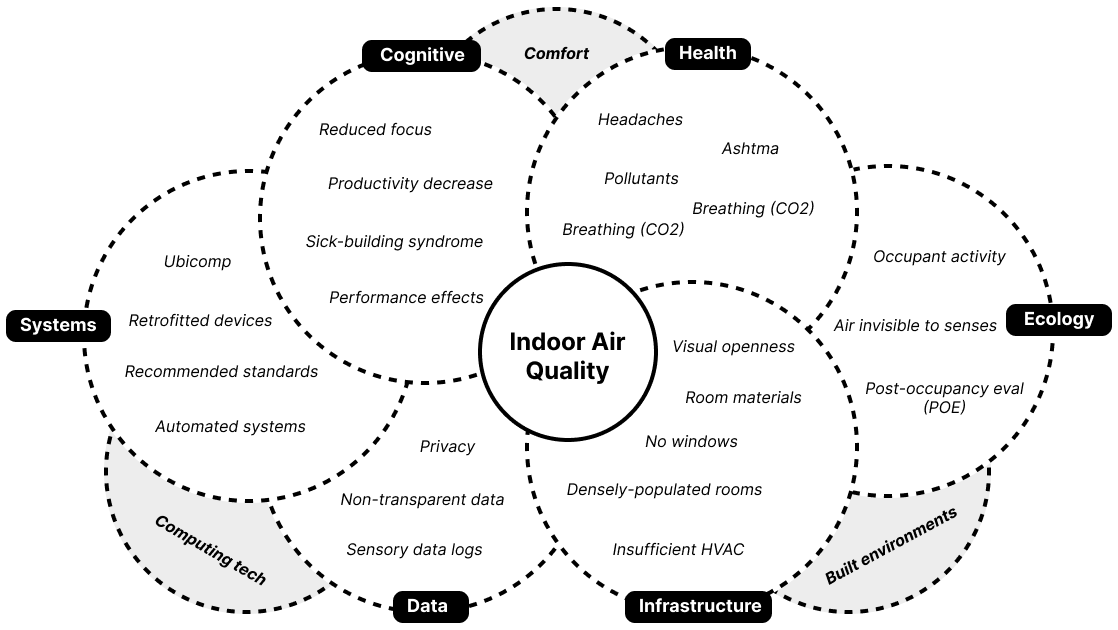
\includegraphics[width=0.5\textwidth]{complexity_diagram_indoor_air_quality.png}
    \caption{Development of the concepts and sketches}
    \label{fig:complexity}
\end{figure}

\subsection{Evaluation}

The prototype was evaluated using common performance-related criteria that are widely used in HCI/Information Visualisation were also used to evaluate the data physicalization prototype \cite{ranasinghe_encoding_2023}. We employed a field-based evaluation approach with accompanying methods based on the Ideo Design Kit \cite{} and Delft Design Guide \cite{}.

\subsubsection{Semi-structured interviews}

Performed semi-structured interviews with self-developed questionnaires.

\subsubsection{Live user observation}

Performed a field trial by observing users in the meeting rooms and interacting with the prototype think aloud.